%%%%%%%%%%%%%%%%%%%%%%%%%%%%%%%%%%%%%%%%%
% Beamer Presentation
% LaTeX Template
% Version 1.0 (10/11/12)
%
% This template has been downloaded from:
% http://www.LaTeXTemplates.com
%
% License:
% CC BY-NC-SA 3.0 (http://creativecommons.org/licenses/by-nc-sa/3.0/)
%
%%%%%%%%%%%%%%%%%%%%%%%%%%%%


%----------------------------------------------------------------------------------------
%	PACKAGES AND THEMES
%----------------------------------------------------------------------------------------

\documentclass[aspectratio=169]{beamer}



\DeclareMathOperator*{\argmin}{arg\,min}


%%%%%%%%%%%%%

\usepackage{hyperref}


\newcommand{\bi}{\begin{itemize}}
\newcommand{\ei}{\end{itemize}}
\newcommand{\m}{\item}
\newcommand{\be}{\begin{enumerate}}
\newcommand{\ee}{\end{enumerate}}
\newcommand{\al}{\alert}
\newcommand{\ul}{\underline}


\mode<presentation> {


\usetheme{Frankfurt}

% As well as themes, the Beamer class has a number of color themes
% for any slide theme. Uncomment each of these in turn to see how it
% changes the colors of your current slide theme.



}


%{%
%}

\setbeamercolor{section in head/foot}{bg=lightgray} %set the top navigation bar background color
\setbeamertemplate{footline}[frame number] % set frame page number only
\usepackage{appendixnumberbeamer} % total will not include appendix frame numbers 

\beamertemplatenavigationsymbolsempty



\usepackage{graphicx} % Allows including images
% graphicx also allows for resizebox
% graphicx also allows for \scalebox
\usepackage{caption}
\usepackage{subcaption} % packgage for subcaption in subfigures
% The subfig and subcaption packages can not be used in cooperation with each other. Instead, you can usecaption package with subfig to add some flavor to the captions and subcaptions
\usepackage{bm} % make bold math symbols
\usefonttheme{professionalfonts}
\usepackage{tabularx} % extra features for tabular environment
\usepackage{booktabs} % Allows the use of \toprule, \midrule and \bottomrule in tables
\usepackage{adjustbox} % allows adjustbox
\usepackage{amsmath}  
\usepackage{amsfonts}
\usepackage{hyperref} % package for hyper link

% the following hypersetup makes link blue
\hypersetup{
  colorlinks   = true, %Colours links instead of ugly boxes
  urlcolor     = blue, %Colour for external hyperlinks
  linkcolor    = blue, %Colour of internal links
  citecolor   = blue %Colour of citations
}


\usepackage{float} % make the table H effective
\restylefloat{table}
\usepackage{color, colortbl}
\usepackage{booktabs} % package for tex professional table
\usepackage{mathtools} % package for \coloneqq
\usepackage{multirow} % multirow for intuition page.

% make pdf dark mode

\usepackage{pifont}% http://ctan.org/pkg/pifont
\newcommand{\cmark}{\ding{51}}%
\newcommand{\xmark}{\ding{55}}%



\usepackage{tikz} % graph in latex
\usetikzlibrary{positioning,arrows.meta} %tikz diagram
\usepackage{pgfplots}
\pgfplotsset{compat=newest} %this setting allow node to go to the correct place
\usepgfplotslibrary{fillbetween}

% use the tikz external library to cache tikz drawings
\usetikzlibrary{external}
\tikzexternalize[prefix=tikz/,optimize command away=\includepdf]



\usepackage{natbib} % package for citation


\usepackage{multicol}


% The subfig and subcaption packages can not be used in cooperation with each other. Instead, you can usecaption package with subfig to add some flavor to the captions and subcaptions


% define a comment line that does nothing to hide content
\newcommand{\comment}[1]{}
\newcommand{\lnb}[1]{%
  \ln\left(#1\right)%
}
\renewcommand{\baselinestretch}{1.0} %  scales the default interline space to 1.0 its default value. 

% define a comment that can scale the equation 
\newcommand\scalemath[2]{\scalebox{#1}{\mbox{\ensuremath{\displaystyle #2}}}}

%----------------------------------------------------------------------------------------
%	TITLE PAGE
%----------------------------------------------------------------------------------------

\title[Prediction Markets]{\huge{Prediction Markets} \\
\vspace{6mm}
\small{MGT 4074 Fintech \& Crypto Tokens, Fall 2025}
} % The short title appears at the bottom of every slide, the full title is only on the title page




\author[Joseph Hall]{Joseph Hall} % Your name
\institute[GT]{Georgia Institute of Technology} % Your institution as it will appear on the bottom of every slide, may be shorthand to save space
 % Your institution for the title page
 % Your email address
 
\date{October 22, 2025} 
 % Date, can be changed to a custom date if without date



%---------------------------------------------------------------------------
\begin{document}

\newcolumntype{d}[1]{D{.}{.}{#1}}


\begin{frame}
\titlepage % Print the title page as the first slide
\end{frame}


%----------------------------------------------------------------------------------------

%	PRESENTATION SLIDES
%----------------------------------------------------------------------------------------

%-----------------------------------------------



%---------------------------------------------------------------------
%---------------------------------------------------------------------
%---------------------------------------------------------------------
%---------------------------------------------------------------------



\begin{frame}{Welcome! Today is Wednesday 10/22/2025}
\begin{center}
\vfill 
The final project proposal deadline has been delayed to \textbf{tomorrow at noon}.\\ Stay tuned for feedback and the presentation schedule, which will be released by Monday 10/27. \\ \vfill 

I will also clarify the \textbf{AI Policy for Final Projects}: yes you may use AI! You are responsible, however, for understanding every part of your final submission from the code to the presentation. If I ask you how or why you did something in a certain way, ``I don't know, that was AI'' is \textbf{NOT} an acceptable answer. 
\vfill 
\end{center}

\end{frame}


\begin{frame}
\frametitle{Roadmap}
\tableofcontents
\end{frame}

%------------------------------------------------

%------------------------------------------------
% insert table of content before each section or subsection
%------------------------------------------------
\AtBeginSection[]
{
\begin{frame}
\frametitle{Roadmap}
\tableofcontents[currentsection]
\end{frame}
}

\AtBeginSubsection[]
{
\begin{frame}
\frametitle{Roadmap}
\tableofcontents[currentsection,currentsubsection]
\end{frame}
}
%------------------------------------------------

\section{In the News}


\begin{frame}{AWS Outage Breaks the Internet}
      \centering
 \hfill 
  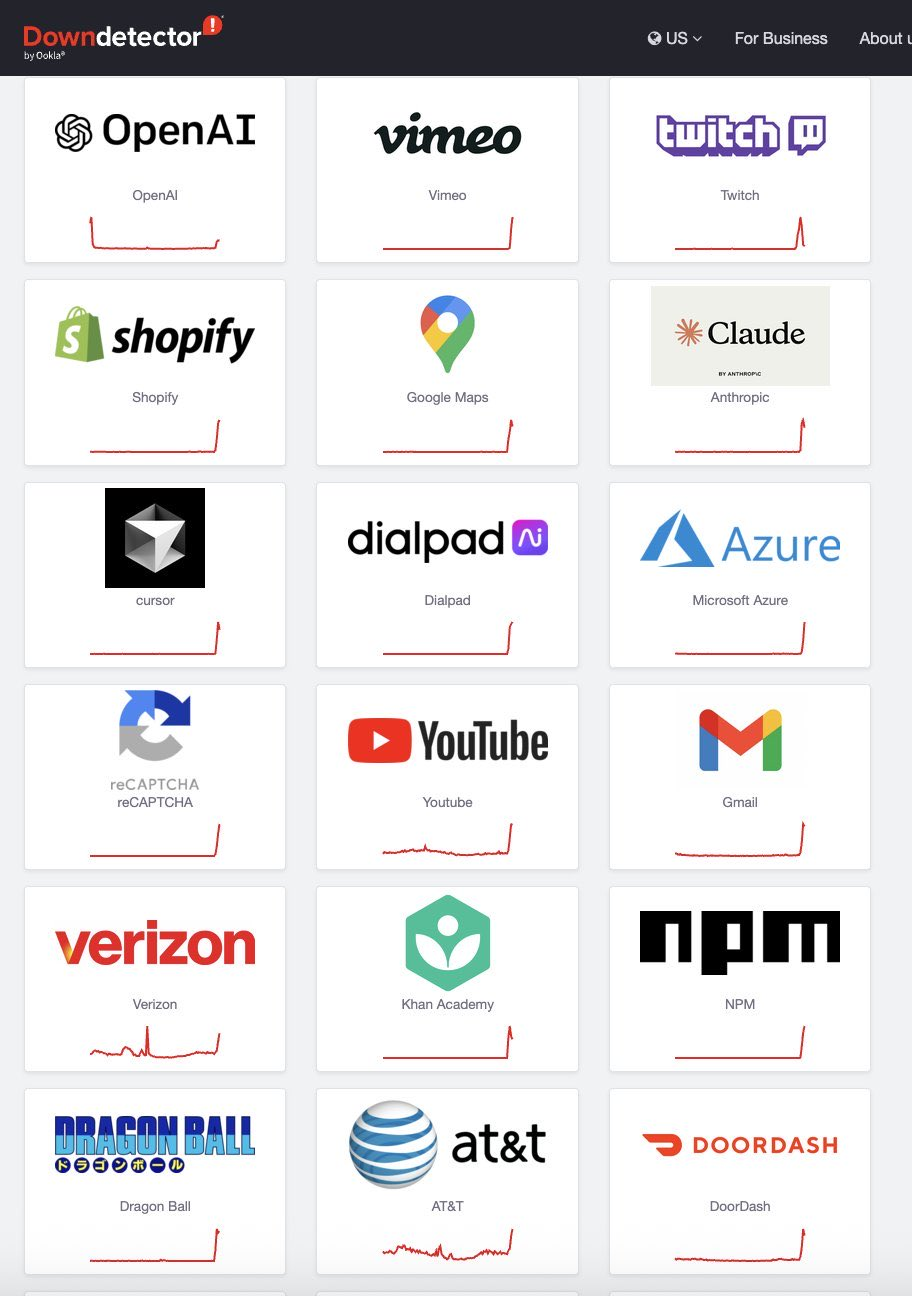
\includegraphics[width=0.35\textwidth]{awsdown1.jpeg}
  \hfill
  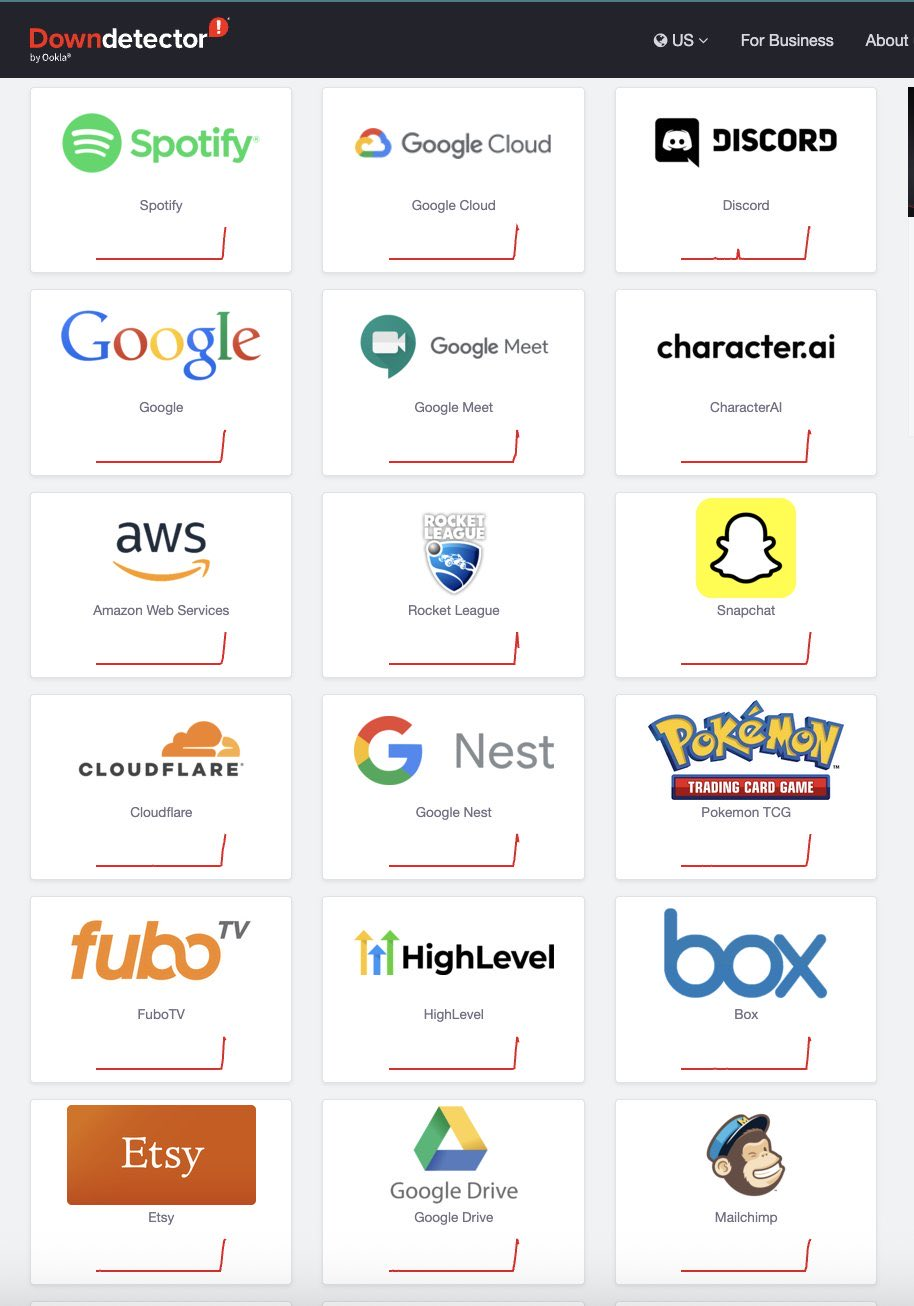
\includegraphics[width=0.35\textwidth]{awsdown2.jpeg}
  \hfill 

\end{frame}


\begin{frame}{Impact of Cloud Service Outage on DeFi}

\centering\hfill 
    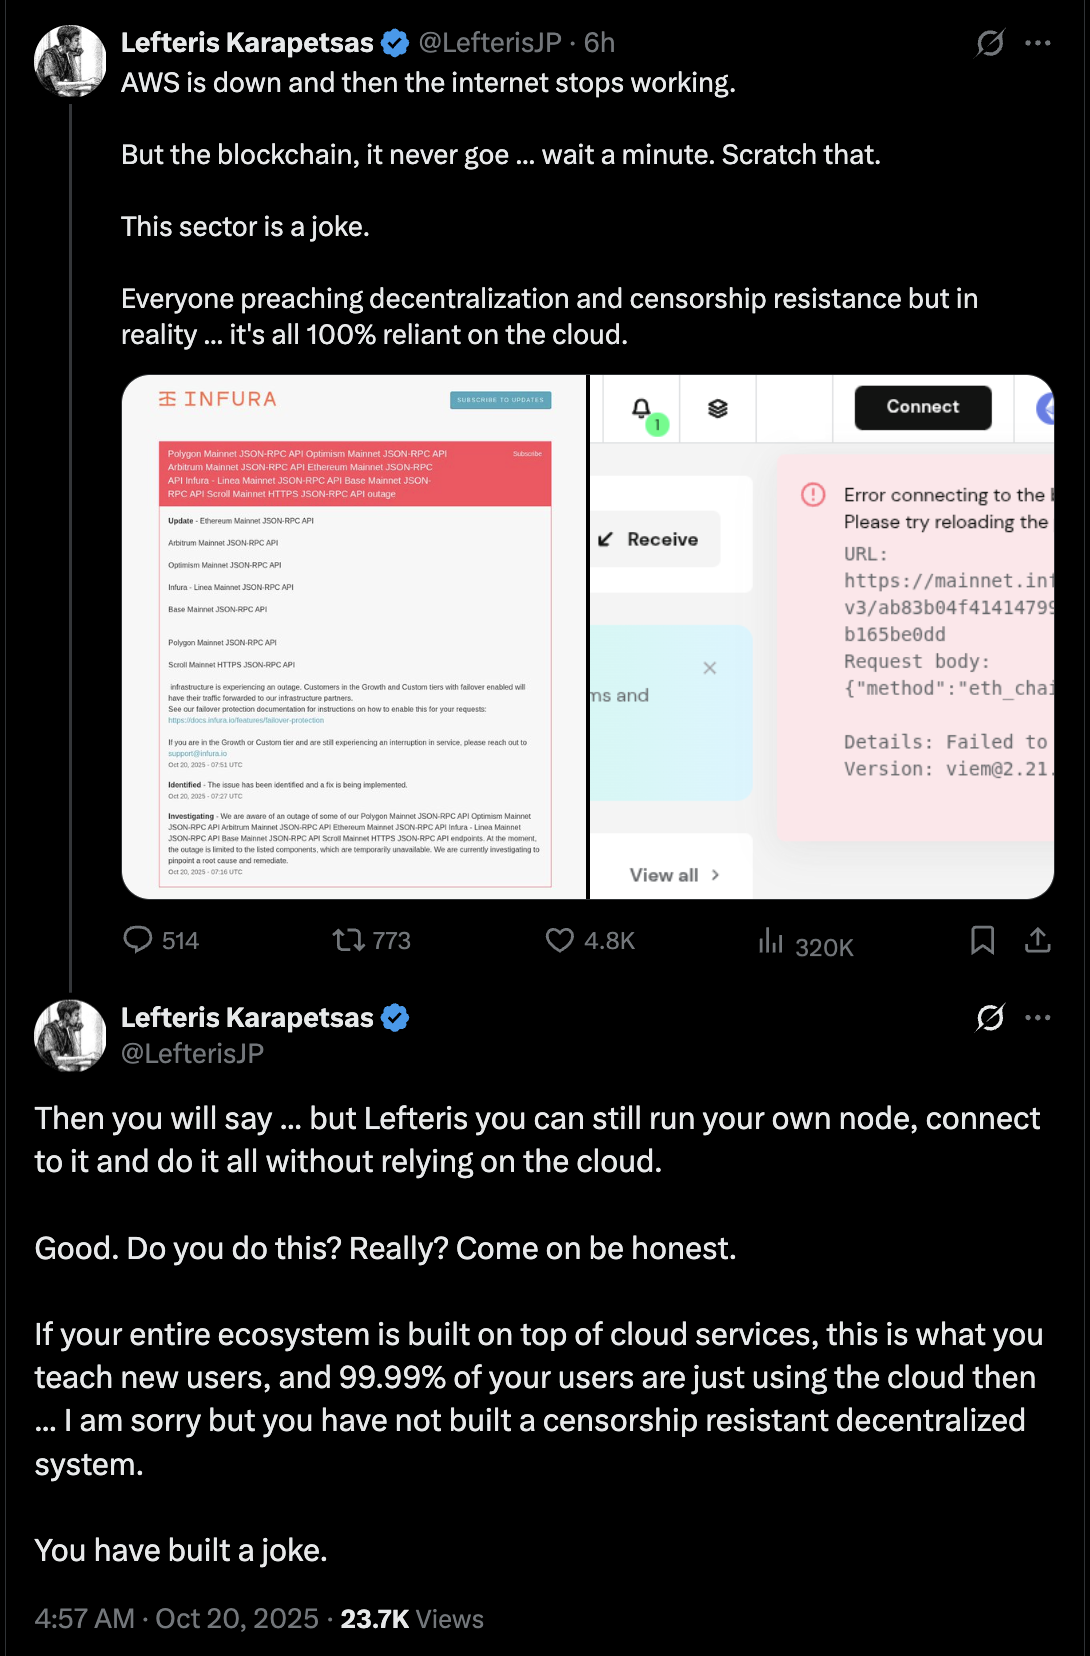
\includegraphics[width = .3\textwidth]{lefteris.png} \hfill 
    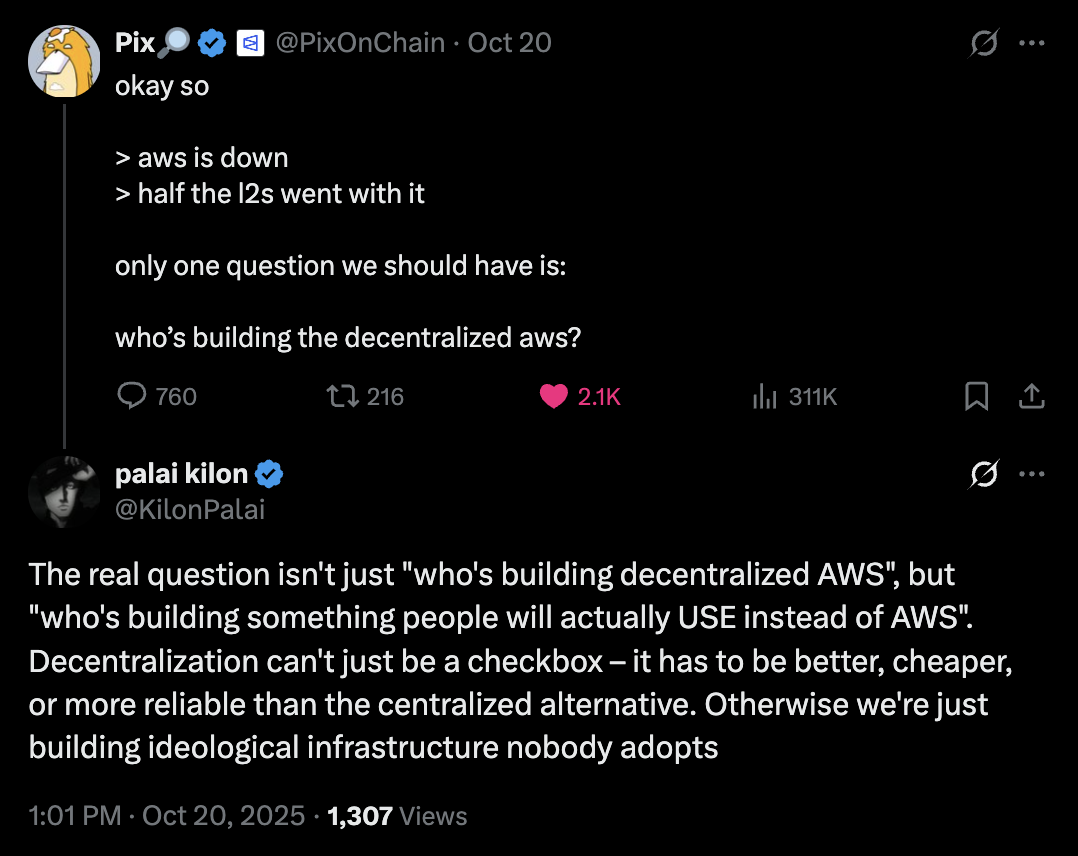
\includegraphics[width = .5\textwidth]{pix.png}\hfill 

    
\end{frame}


\section{Prediction Platforms}

\begin{frame}{Definition}

In a \textbf{Prediction Market}, bets are traded on binary outcomes: \$1 if prediction comes true, \$0 if prediction does not. \\ 

There are two major market structures of prediction markets: 

\bi 
\m  In \textbf{Proprietary} markets, one entity (``the house'') lists odds unilaterally and takes the opposite side of every customer's bet. 
\bi 
\m These are often called ``sportsbooks'', ``bookies'', ``oddsmakers'' or just ``Vegas''. 
\m The prices offered for complementary predictions add up to much more than \$1 - there is a ``house edge'' which is called a ``vig'' or ``juice'' 
\m The house usually tries to match its book (sell equal quantities of yes and no) -- ``the house always wins'' \pause 
\ei 
\m In \textbf{Peer to Peer} markets, opposite sides of the bet must match exactly and agree on a market price to create a bet. 
\bi 
\m Kalshi uses a P2P structure despite being a centralized platform; it takes a transparent fee instead of a house edge 
\ei 
\ei 

\end{frame}


\begin{frame}{Behavior in Prediction Markets}

From \href{https://mattbrownecon.github.io/assets/papers/jmp/sportsbetting.pdf}{Matt Brown Econ}: 
\begin{itemize}
    \item The average sports better is \emph{highly overconfident:} They expect to break even (and enjoy the variance) but in fact lose 7.5 cents on the dollar: 
    \item Overoptimism is worse among bettors who prefer \textbf{parlays}: compound bets that all of several (usually uncorrelated) events (``legs'' of the parlay) will all occur successfully with no failures 
    \item Summarizing bettors' historical performance does nothing to correct their bias, but allowing them to set limits in advance reduces gambling by a modest amount 
\end{itemize}
Worldwide, about 60\% of gambling losses (aka gambling industry profits) come from gambling addicts \href{https://www.who.int/news-room/fact-sheets/detail/gambling}{per the World Health Organization}. 
    
\end{frame}


\begin{frame}{Popular Prediction Markets}

Popular prediction markets include: %today vary by \textbf{centralization}, \textbf{regulation}\footnote{CFTC generally does not regulate decentralized exchanges}, \textbf{event categories} and \textbf{for-profit status}: 

\bi 
\m \textbf{Kalshi}, a centralized and regulated for-profit all-purpose prediction market 
\m \textbf{Polymarket}, a decentralized and unregulated all-purpose prediction market 
\m \textbf{Predictit}, a centralized and regulated non-profit prediction market focused on political outcomes 
\bi 
\m I dabbled in Predictit in college, but it was impossible to make money after fees 
\ei 
\m Several other exchanges, mostly sportsbooks (\textbf{ESPNBet}, \textbf{DraftKings}), have grown rapidly since the Supreme Court legalized sports gambling in 2018 \pause 
\ei 

Economists love prediction markets for the same reason we love stock markets: they incentivize people to \emph{gather and reveal information} that the rest of us get \emph{for free!}

\end{frame}

\begin{frame}{Polymarket Growth}

\begin{center}
    \href{https://dune.com/queries/3996727/6732246}{Polymarket Monthly Volume}
\end{center}

\bi
\m Since Polymarket is on-chain, Dune can make an easy dashboard! 
\m Dune uses Structured Query Language (SQL), which you should learn if you haven't already (it's incredibly easy) 
\m \href{https://tpan.substack.com/p/381-the-grand-integration-of-prediction}{TPan on Substack}
\ei 
    
\end{frame}


\begin{frame}{Illegal Event Categories}

A prediction is a type of derivative. Many derivative markets are \emph{per se}\footnote{Legal term: ``Without determination by or involvement of extraneous factors; by its very nature.''} illegal! \pause 

\bi 
\m Predicting the death of individuals 
\bi 
\m A popular financial product was once the \textbf{Tontine}: a group pools funding, and each receives annuity payouts until they die. Payouts increase as one outlive their peers 
\m The reason should be obvious: it creates incentives for murder \pause 
\ei 
\m \textbf{Motion Picture Box Office Receipts}: Swept up in 2008 Dodd-Frank \href{https://www.theringer.com/2018/11/15/movies/box-office-futures-dodd-frank-mpaa-recession}{(story)}
\m \textbf{Onion Futures}, banned by Congress in 1958 in response to the Great Onion Corner of 1955 where one man came to own every onion in Chicago and was able to extort wholesalers 
\ei 
Prediction markets are not regulated by the SEC, but rather the \textbf{Commodities Futures Trading Commission (CFTC)}. Predictions (about things that aren't securities) are considered ``Arrow Securities'' by academics, but ironically are \underline{not} considered ``securities'' by U.S. law! (who remembers the \emph{Howey Test}?) 
    
\end{frame}


\begin{frame}{CFTC Signals Support for Decentralized Markets}
    \begin{center}
        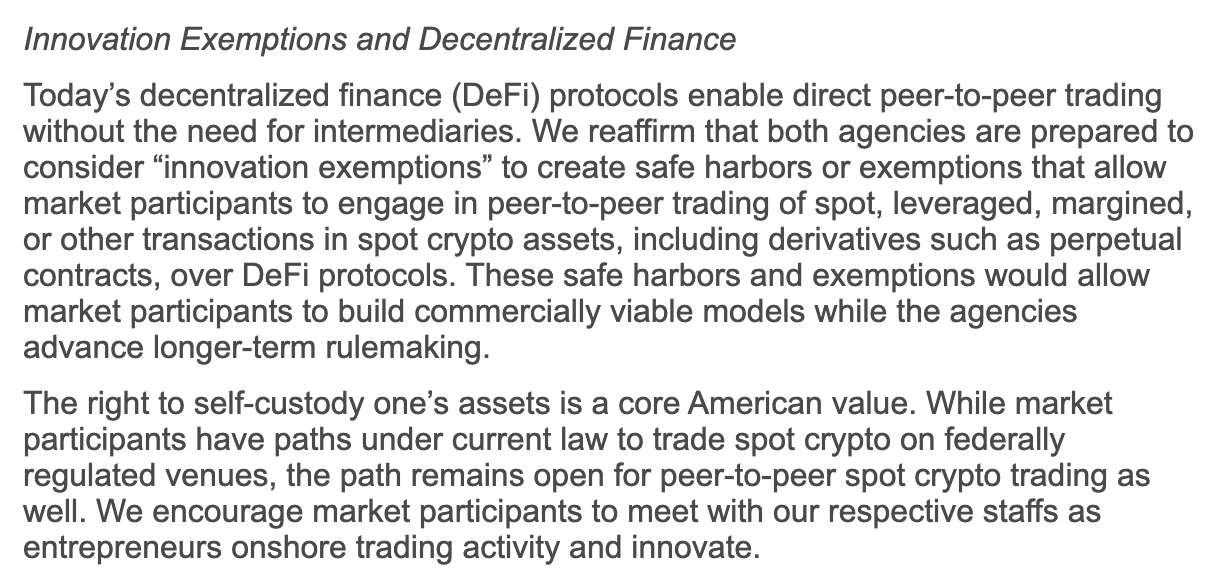
\includegraphics[height = .8\textheight]{cftc.png}
    \end{center}
\end{frame}


\section{Gambler's Math}


\begin{frame}{Odds and Prices}

Sports books list prices using \textbf{Moneyline Odds}: 

\bi 
\m \textbf{Plus odds}\footnote{or ``long odds'' as the popular expression goes} are prices below 50 cents: ``+300'' means \pause bet \$100 to win \$300, which corresponds to a price of \pause  25 cents
\bi 
\m Use the formula $\frac{100}{100+X}$ to convert odds of $+X$ to a price \pause 
\ei 
\m \textbf{Minus odds} are prices above 50 cents: ``-300'' means bet \$300 to win \$100, which corresponds to a price of 75 cents 
\bi 
\m Use the formula $\frac{X}{100+X}$ to convert odds of $-X$ to a price 
\ei 
\ei 
\pause 
The \textbf{Moneyline} is contrasted with the \textbf{Spread}, which is an equal-odds bet on the margin of victory. When two teams are unevenly matched, the ``line'' can be ``drawn'' in probability space (the ``moneyline'') or in margin-of-victory space (the ``spread'')\footnote{You could equivalently call it the ``pointsline''} 

\end{frame}

\begin{frame}{Example: ATL vs. MIA, Oct 26 2025}

What is the implied probability that the Atlanta Falcons defeat the Miami Dolphins? 

\begin{center}
    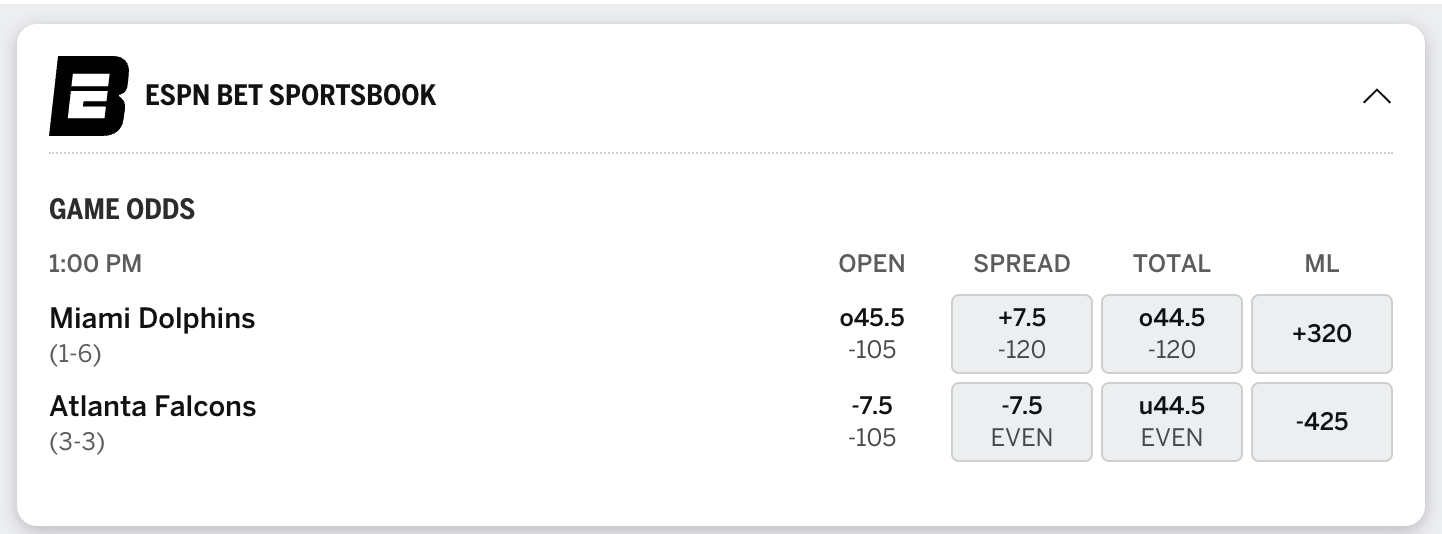
\includegraphics[width = .9\textwidth]{espn_bet.png}
\end{center}
    
\end{frame}


\begin{frame}{Example: ATL vs. MIA, Oct 26 2025}

Use the odds-price formula: 
\bi 
\m The \textbf{Miami Dolphins} are $+320$: $\frac{100}{320+100}=24\%$ \pause 
\m The \textbf{Atlanta Falcons} are $-425$: $\frac{425}{425+100}=81\%$
\ei 
\textbf{Q:} Why do these numbers not add up to 100\%? \\  \pause 
\textbf{Hint:} It's not because of the possibility of a tie -- that should causee them to add up to \textbf{less than 100\%}!  \\ \pause 
\textbf{A:} This is the \textbf{House Edge}: in this case $24\%+81\%-100\% = 15\%$ \\ \pause 
\textbf{Q:} Why do they list it this way? \\ \pause 
\textbf{A:} To confuse you and hide the house edge. 
    
\end{frame}



\begin{frame}{Kelly Criterion}

The \textbf{Kelly Criterion} is a formula, derived using basic statistics and calculus, to determine how large of a wager to make (``\textbf{bet sizing}'')
\vfill 
The Kelly Criterion \emph{assumes} you have an \textbf{edge}: you know that the true probability is different from the market-implied probability \pause 
\vfill \pause 
The Kelly Criterion is ``edge over odds'': 

$$\frac{\mathrm{edge}}{\mathrm{odds}} =\frac{E[\mathrm{profit\,per\,\$1\,bet}]}{\mathrm{odds\,ratio}}$$
\pause 

E.g. You are offered 5-to-1 odds (wager \$1 to win \$5 (collect \$1+\$5=\$6)), but you know the event has a 50\% true probability. On average, you collect $50\%\times\$6=\$3$ for an ``edge'' of $\$3-\$1=\$2$. The formula is therefore $2/5=40\%$: you should wager 40\% of your wealth on that bet. 
\vfill \pause 
It maximizes expected wealth over many \textbf{independent (uncorrelated) bets} 

\end{frame}


\begin{frame}{Prices and Probabilities}

The price (e.g. 90 cents) of a prediction market asset is often called the probability. \pause While accurate for petty gambling, this can be incorrect for two reasons: 

\bi 
\m \textbf{Time Value of Money} -- the asset is traded today but the payoff of the bet might be a long time from now (e.g. 2028 Presidential Election), necessitating an adjustment for time value of money. \pause 
\m \textbf{State Prices} -- Predictions strongly correlated with macroeconomics can trade above or below probability because of \textbf{state prices}: a dollar in the state of the world where we have a recession becomes especially valuable. Therefore that prediction will trade \underline{above true probability}. 
\ei 

The second term is not generally possible to calculate without strong assumptions. The first term is easy -- just inflate the price by the time value (e.g. maturity-matched treasuries) between the trade date and the settlement date to get the probability. \textbf{For bets resolving in the near future and uncorrelated with the macroeconomy, prices in a frictionless competitive market should trade to true probability}
    
\end{frame}

\section{Decentralized Prediction Markets}


\begin{frame}{Polymarket}

\begin{center}
    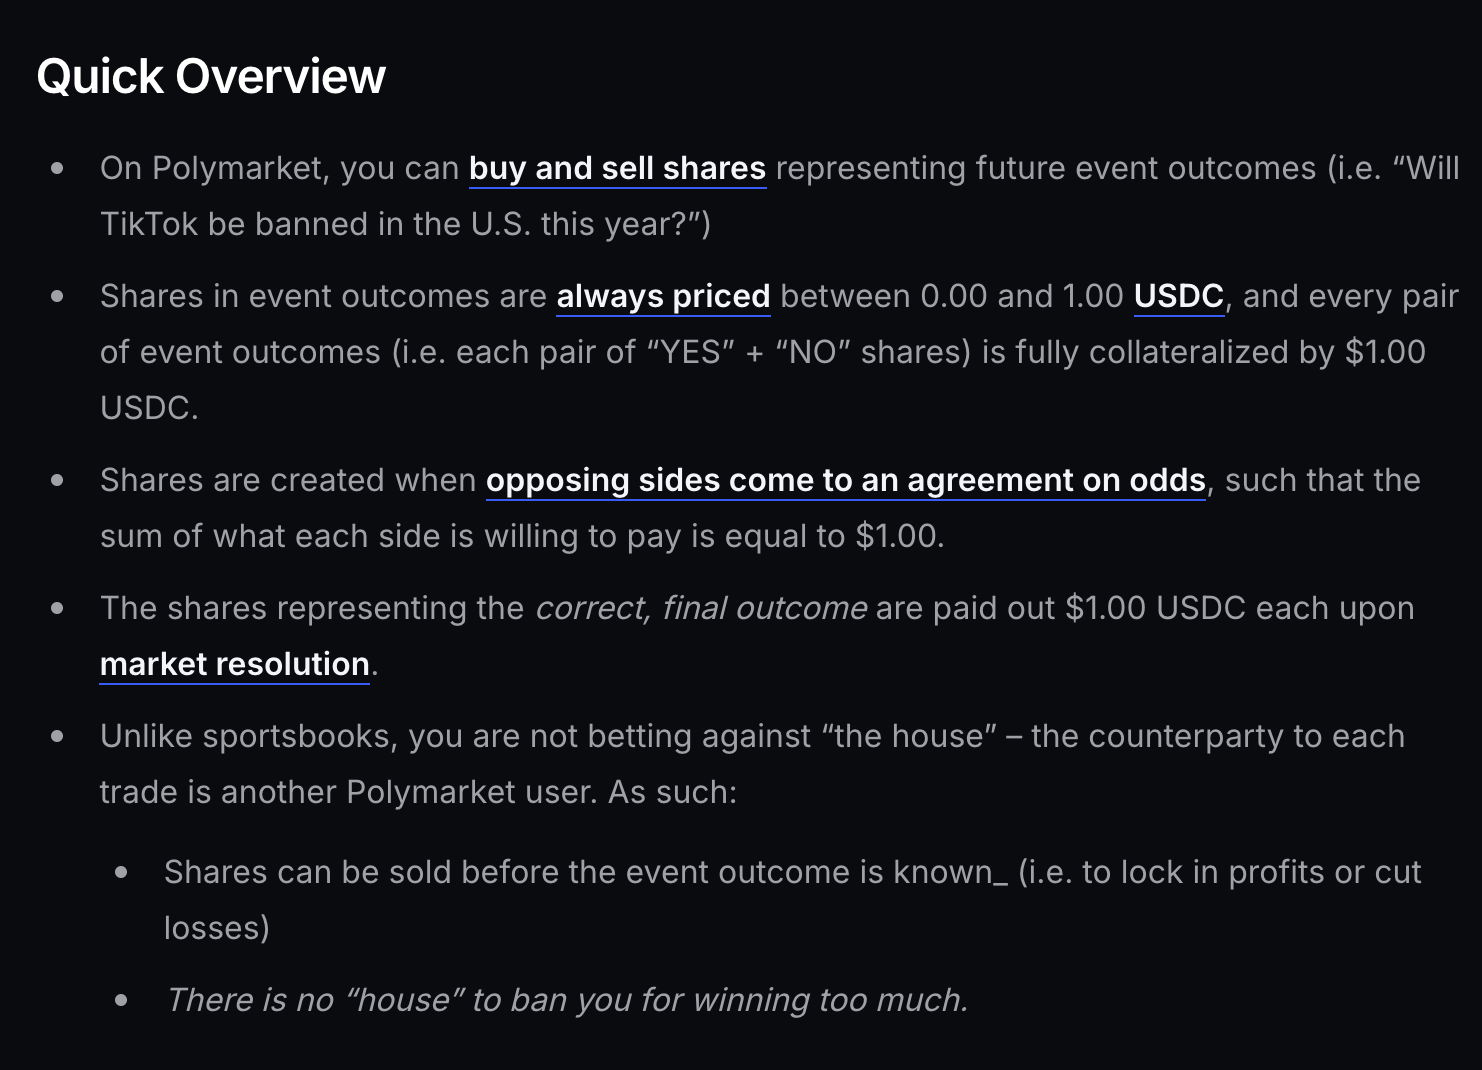
\includegraphics[height = .8\textheight]{polymarket_overview.png}
\end{center}
    
\end{frame}

\begin{frame}{Polymarket vs. Sportsbook ``House Edge''}

\begin{center}
    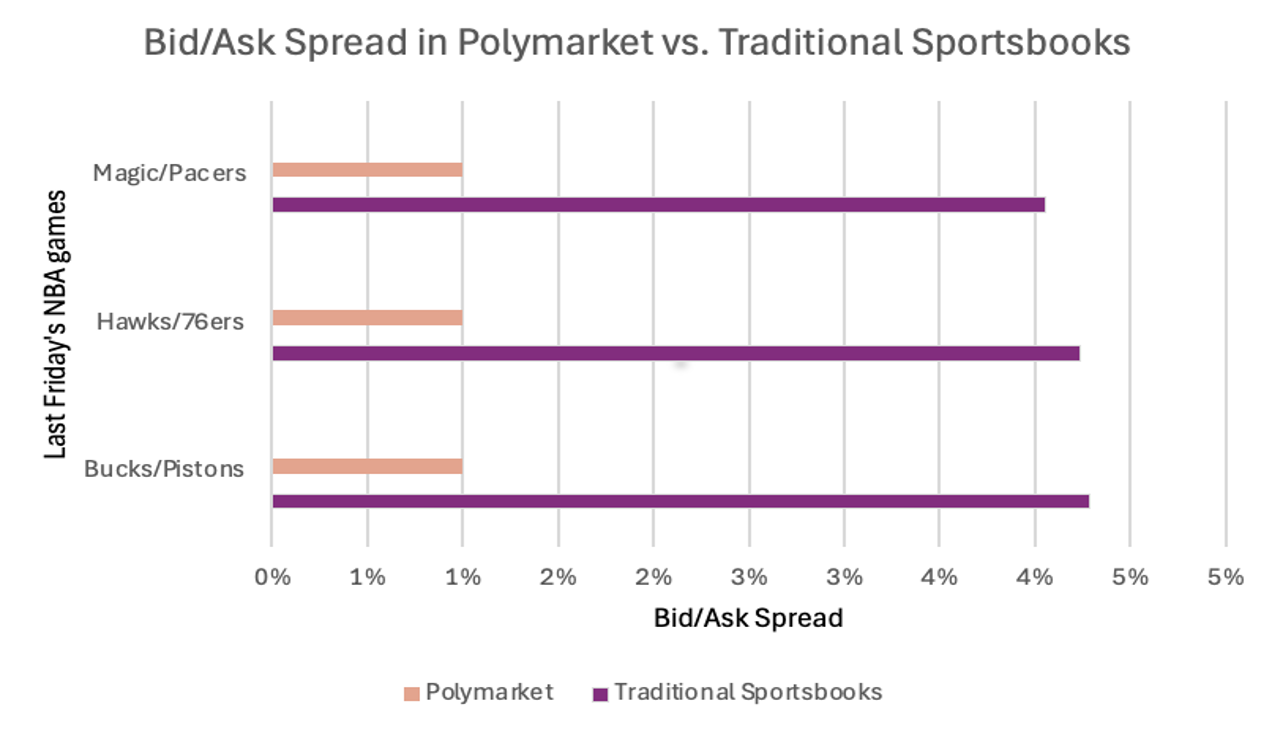
\includegraphics[height = .8\textheight]{bognar_polymarket.png}
\end{center}

Source: Nils Bognar, MGT4074 Spring 2025 Final Project
    
\end{frame}


\begin{frame}{Oracle Risk in Decentralized Markets}

Just as in all other decentralized markets, decentralized prediction markets are heavily exposed to \textbf{Oracle Risk}: the chain has no eyes of its own and must be told what has occurred in the real world. \\

Polymarket uses the \textbf{UMA Optimistic Oracle} to resolve bets. \pause 
\bi 
\m ``Optimistic'' means that users put down collateral to propose to resolve outcomes. The collateral is lost if their proposed resolution is successfully challenged. 
\m UMA is the governance token for the optimistic oracle. \emph{Owners of UMA tokens comprise the ``jury'' in the case of any dispute}
\ei 
If you own a majority of UMA Tokens, you can rig the oracle! The creators of UMA call this ``profit-from-corruption'' or ``PFC'' risk in their \href{https://github.com/UMAprotocol/whitepaper/blob/master/UMA-DVM-oracle-whitepaper.pdf}{whitepaper}. 
    
\end{frame}

\begin{frame}{UMA Optimistic Oracle}

\begin{center}
    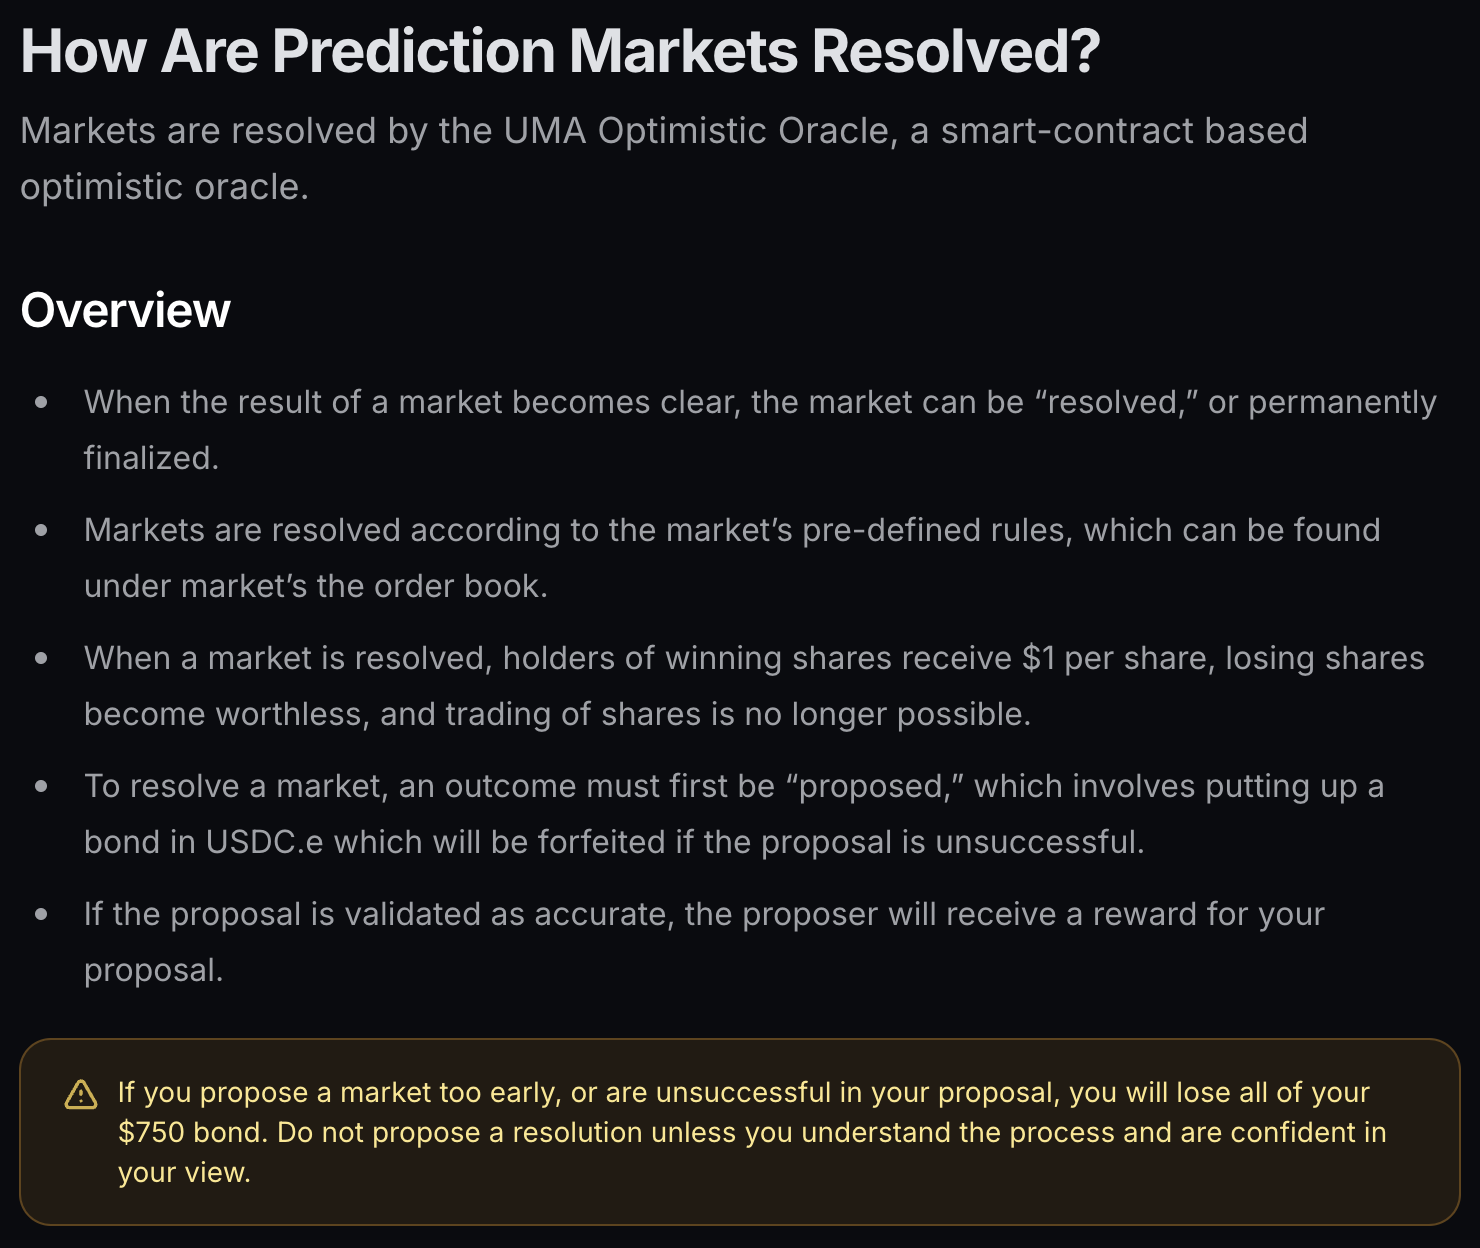
\includegraphics[height = .8\textheight]{polymarket_resolution.png}
\end{center}
    
    
\end{frame}


\begin{frame}{Polymarket Oracle Failure}

\begin{center}
    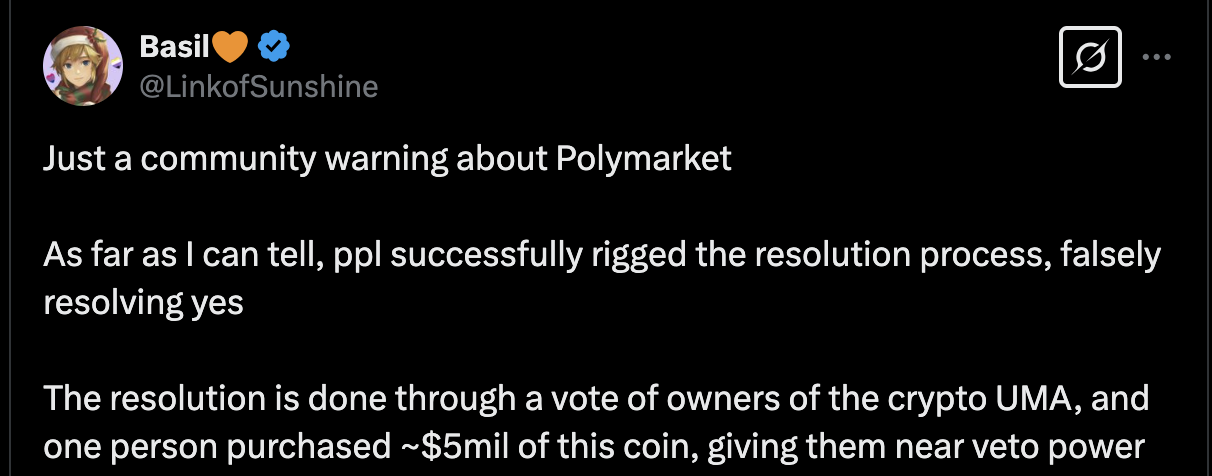
\includegraphics[width = .9\textwidth]{polymarket_tweet.png}
\end{center}
    
\end{frame}


\begin{frame}{Polymarket Oracle Failure}

\begin{center}
    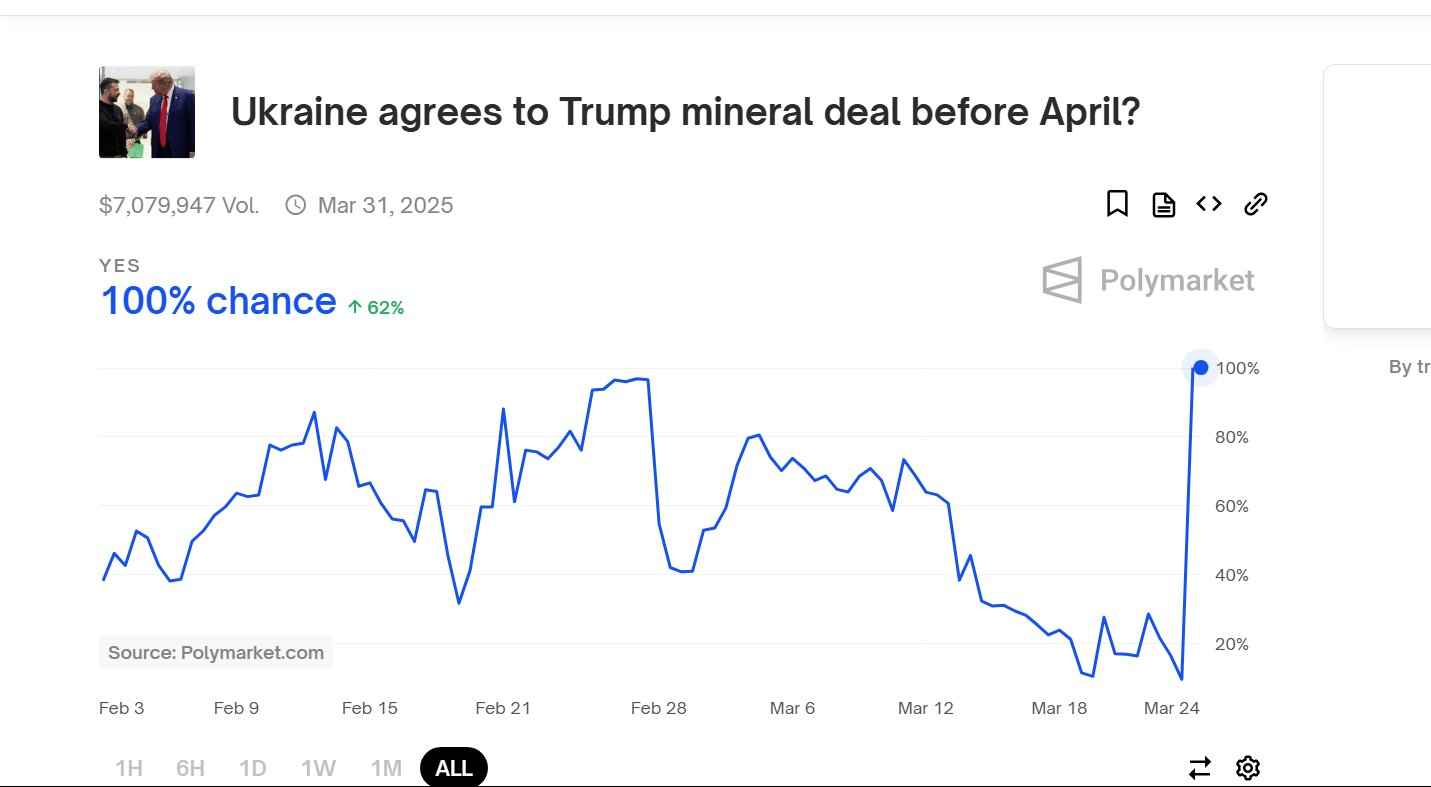
\includegraphics[height = .8\textheight]{polymarket_ukraine.png}
\end{center}
    
\end{frame}


\begin{frame}{Polymarket Oracle Failure}

\begin{center}
    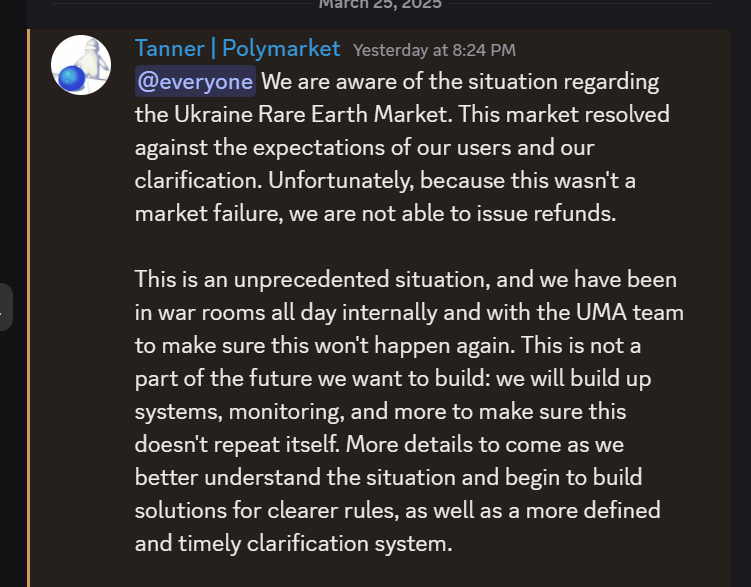
\includegraphics[height = .8\textheight]{polymarket_discord.png}
\end{center}
    
\end{frame}


\end{document}
